\chapter{Data Processing}

In this chapter, we discuss the data processing steps that are required to prepare the data for the model development process. Firstly, we address different session parameters and how they might influence the data. Secondly, we explain the data acquisition process and how the data is stored in files such that it can be used in the future. Thirdly, we discuss the data population process in which the human pose data is extracted from the raw data. To ensure the quality of the dataset we then evaluate the data by filtering invalid skeletons and marking data points as valid or invalid. Finally, we discuss the data augmentation process in which the data is augmented to increase the size of the dataset.

\section{Developed Software}

\textit{\textbf{UNSURE} Should I write about the software, explain the OpenGL implementation, the ImGui GUI and so on?}
\textit{\textbf{TODO} Change Screenshots to light mode to be consistent with the rest of the thesis (can wait until screenshots are final)}

\begin{figure}[ht]
  \centering
  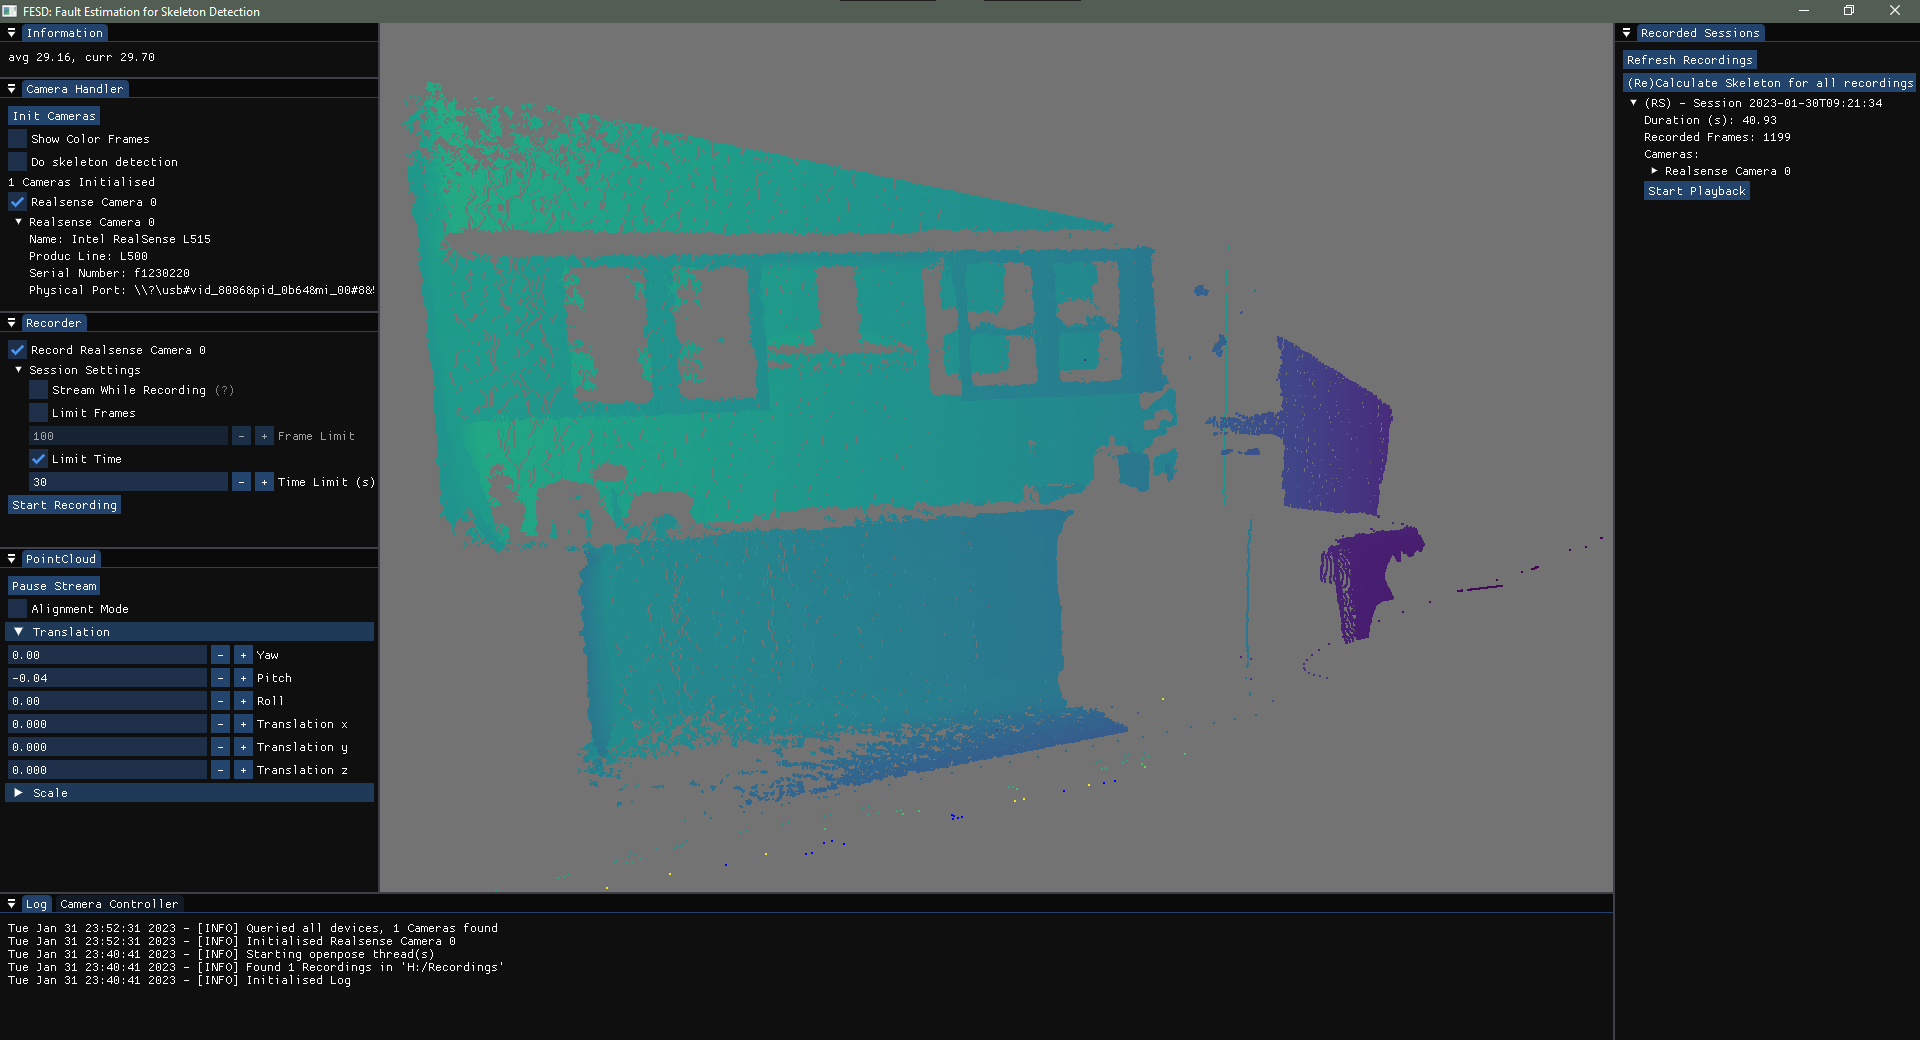
\includegraphics[width=\linewidth]{figures/FESD/all.png}
  \caption[FESD GUI]{A screenshot of the FESD GUI streaming a point cloud. The GUI is used to record and visualize the data, and to playback recordings to validate the data. The GUI is written in C++ using the ImGui framework. The Pointcloud is visualised using OpenGL and a glsl shader.}
  \label{fig:stream_gui}
\end{figure}